
%\documentclass{article}
\documentclass[11pt, oneside]{amsart}
\usepackage[bottom=1.25in]{geometry}
\usepackage[utf8]{inputenc}
\usepackage[parfill]{parskip}    % Activate to begin paragraphs with an empty line rather than an indent
\usepackage{graphicx}
\usepackage{amssymb}
\usepackage{epstopdf}
\usepackage{tabu}
\usepackage{booktabs}
\usepackage{etoolbox}

\usepackage{graphicx}
\usepackage{dcolumn}
\usepackage{booktabs}
\usepackage{amsmath}
%\usepackage{amssymb}
\usepackage{pxfonts}
%\usepackage[a4paper, total={6in, 8in}]{geometry}
%\usepackage{lineno}

%\usepackage{lineno}
%\usepackage{fancyhdr}

\pagestyle{plain}
%\pagestyle{fancy}
%\lhead{Electronic Supplemental Material}
%\rhead{Humphrey \emph{et al.}}
%\cfoot{\thepage}

%\DeclareGraphicsRule{.tif}{png}{.png}{`convert #1 `dirname #1`/`basename #1 .tif`.png}
%\DeclareMathOperator{\logit}{logit}
%\newcommand{\lib}[1]{\texttt{#1}}
%\renewcommand{\thetable}{S\arabic{table}}
%\renewcommand{\thefigure}{S\arabic{figure}}
%\newcommand\tab[1][0.75cm]{\hspace*{#1}}

\title{\textbf{Appendix S3}}
\author{\emph{Ecosphere}\\
\\
\text{Habitat preference of an herbivore shapes the habitat distribution of its host plant}
\\
\\
Nicolas M. Alexandre, Parris T. Humphrey, Andrew D. Gloss, Jimmy Lee, Joseph Frazier, Henry A. Affeldt III, and Noah K. Whiteman.\\
\\
\textbf{Statistical Supplement}}
%\author{\emph{Alexandre, Humphrey et al.}}
\date{25 July 2018}

\DeclareMathOperator{\logit}{logit}
\newcommand{\ltfrac}[2]{\mbox{\large$\frac{#1}{#2}$}}
\def\code#1{\texttt{#1}}
\newcommand{\lib}[1]{\texttt{#1}}
\setlength\parindent{0pt}  % sets indent to zero
\setlength{\parskip}{10pt} % changes vertical space between paragraphs
\renewcommand{\thetable}{S\arabic{table}}
\renewcommand{\thefigure}{S\arabic{figure}}

\begin{document}
 \maketitle
 
\tableofcontents

\section{Herbivory survey}
\subsection{Biological motivation}
\label{S:1}
%\linenumbers
%Herbivore damage from \emph{Scaptomyza nigrita} on its host plant, \emph{Cardamine cordifolia} arises from a sequence of contingent events: (i) the arrival by an herbivore, usually a female, at a host plant (or leaf), and (ii) the damage that results from acceptance of such a host by an adult female or a larva. The former process is influenced by local herbivore abundance, which can directly impact the proportion of stems which receive any damage (prevalence). Conditional on an individual herbivore accepting a leaf, the probability that the resulting damage is of a particular extent can also vary among stems and/or sites owing to underlying differences in average palatability of the plants.\

Herbivore damage (in this case, counts of feeding punctures made by adult females ['stipples'], leaf mines made by larvae, and eggs laid by adult females) is typically recorded as positive integer counts, and such count data often exhibit under-dispersion (zero-inflation), over-dispersion (excess variance), or both, with respect to expectations of Poisson or Poisson--Gamma mixture (i.e. negative binomial, NB) models. Our understanding of the foraging ecology of \emph{Scaptomyza nigrita} leads us to expect that dispersion of both of these types is likely. Female flies are choosy, often visiting several leaves before making feeding punctures; females may also avoid leaves entirely, either actively or due to stochasticity in the host sampling process, and local abundances of foraging \emph{S. nigrita} may vary across sampling locations. All three processes can affect the prevalence of damage among leaves and can lead to under-dispersion, and the extent to which this is observed may well vary among sites or habitat types.

In addition, once a host has been preliminarily accepted, we expect that variation in the intensity of feeding damage arises from factors perceived subsequent to the initiation of damage. We thus assume that separate (but potentially related) biological processes govern the host acceptance versus the host damage stages of herbivory as measured in our study, and this also may vary across plants, site or habitat type. Below, Figure \ref{fig:one} shows the distribution of stipple and mine counts from our herbivory survey, broken down by habitat type, and from these raw data plots we can already appreciate the strong difference between habitat types in the prevalence (0 versus $>0$ counts) as well as the average intensity of damage (distribution of counts $>0$).

%%%%% FIG S1
%insert plot!
\begin{figure}[h]
\begin{center}
%\setkeys{Gin}{width=0.5\textwidth}
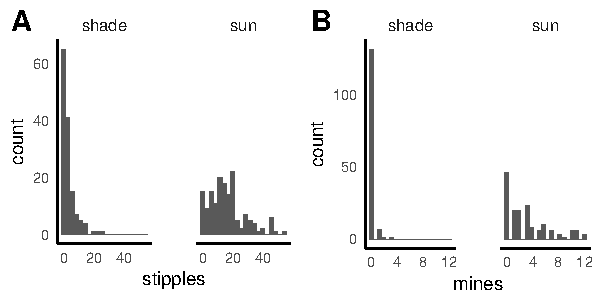
\includegraphics[scale = 0.9]{A3_figS1}
\caption{Distribution of (\textbf{A}) stippling and (\textbf{B}) leaf miner damage on sun and shade-grown bittercress across $n=15$ sites in a field herbivory survey.}
\label{fig:one}
\end{center}
\end{figure}

When we compute the ratio of the variance to the mean for stipple and leaf mine counts for each site (Figure \ref{fig:two}), we observe variation both within and between habitat types. When examining these two figures, we might suspect that a standard Poisson model may be inappropriate for accounting for the range of variation observed in these data, given that we expect the sample variance to sample mean ratio to be $\sim 1$ under a standard Poisson process. Instead, we observe ratios $>1$ and distributions of ratios that differ between site types (Figure \ref{fig:two}; i.e., heteroscedasticity). These two patterns indicate that our count data will \emph{not} be suitably modeled without accounting for zero-inflation and over-dispersion simultaneously. Below we describe our modeling approach for handling dispersion of both types.

%%%%% FIG S2
\begin{figure}[!th]
\begin{center}
%\setkeys{Gin}{width=0.33\textwidth}
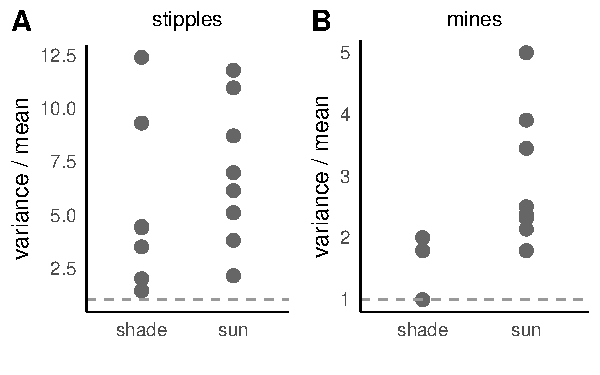
\includegraphics[scale = 0.9]{A3_figS2}
\caption{Variance/mean ratios for (\textbf{A}) stippling and (\textbf{B}) leaf miner damage on sun and shade-grown bittercress. The dashed line indicates unity.}
\label{fig:two}
\end{center}
\end{figure}

%%%%%%% Modeling zero-inflation %%%%%%%%%
\subsection{Modeling zero-inflation}

Zero-inflated models are mixture models composed of a binomial component that models the zero-inflated proportion of the data, and a count component (typically Poisson or NB) that is jointly fit. In such models, the extra zero count compartment results from an inflation of the probability density at $Y=0$ given some unmeasured latent variable that governs the exposure of sampling units to the processes that generate the actual counts \cite{Zuur09a}. When combined with the probability density function of the Poisson distribution, a zero-inflated Poisson becomes

%%% Eq. 1
\begin{equation}
Pr\Big \{Y = y | \theta \Big \} = \begin{cases}
	\pi_{0} + (1 - \pi_{0}) \cdot e^{-\theta}, & \text{if } y = 0.\\
	\\
    (1-\pi_{0}) \cdot \dfrac{\theta^{y}}{y!}e^{-\theta}, & \text{if } y > 0.
	\end{cases}
\end{equation}

where $\theta$ is the Poisson mean and $y$ is an observed count, while the latent variable $\pi_0$ is the probability that a zero count is drawn from the under-exposure sample category rather than from the exposed category of samples. We might wish to describe the influence of habitat type on $\pi_{0}$, and to do so we construct a binomial linear model which estimates the zero-inflation coefficient $\pi_0$ for each habitat type $k$, using the canonical logit link function:

%%% Eq. 2
\begin{equation}
  \logit (\pi_{0}^{k}) = \log \Bigg ( \frac{\pi_{0}^{k}}{1 - \pi_{0}^{k}} \Bigg ) = \begin{cases}
    \delta_0 & \text{if habitat = shade}.\\
    \delta_0 + \delta_1 & \text{if habitat = sun}.
  \end{cases}
\end{equation}

where $\delta_0$ is the estimated coefficient for the shade habitat, taken as the reference level (i.e., the Constant, or Intercept), to which the effect of the sun habitat ($\delta_1$) is added. (Note that the superscript $k$ indicates a group-level index and is not an exponent). In our analysis, we generated maximum likelihood estimates for these ZI parameters using \textbf{R} \cite{R-Core-Team17a} package \lib{glmmTMB} \cite{Jackman15a,Zeileis08a,Loeys12a}. In the main text (Table 1) we report the estimates of $\pi_{0}^{shade}$ and $\pi_{0}^{sun}$ on the probability (i.e. inverse logit) scale along with 95\% (Wald type) confidence intervals.

%\newpage
%%%%%%%%% Modeling the damage intensity process %%%%%%%%%%
\subsection{Modeling the damage intensity process}

Our damage intensity counts are empirically over-dispersed compared to expectations of a Poisson process (Figure \ref{fig:two}). This arises when the variance grows faster than the mean such that variance/mean ratios exceed 1. To accommodate this fact, we model counts of herbivore damage (stipples and leaf mines) as a Poisson random variable ($Y_i$) where the Poisson mean ($\Theta_i$) is itself a random variable. This gives rise to the following expression for the conditional probability of $Y_i$ given $\Theta_i$, in the context of zero-inflation:

%%% Eq. 3
\begin{equation}
Pr\Big \{Y_i = y | \Theta_i = \theta \Big \} = \begin{cases}
	\pi^{k}_{0} + (1 - \pi^{k}_{0}) \cdot e^{-\theta} & \text{if } y = 0\\
	\\
    (1-\pi^{k}_{0}) \cdot \dfrac{\theta^{y}}{y!}e^{-\theta} & \text{if } y > 0
	\end{cases}
\end{equation}

Conceptually, this means that the variance of our random variable $Y$ includes the Poisson variance associated with each Poisson mean $\Theta_i$ as well as additional variance in the distribution of $\theta$ itself. We adopt the conventional probability density function for $\theta$ as a Gamma distribution with scale parameter $\alpha$ and rate parameter $\beta$ \cite{Zuur09a}:

$$g(\theta) = \dfrac{\alpha^\beta}{\Gamma(\beta)}\theta^{\beta-1} \cdot e^{-\alpha \theta}$$

We recover the the unconditional probability of $Y_i$ by integrating out the $\theta$ (i.e. averaging over the distribution of Poisson means) to recover the parameterization of the negative binomial (NB) that we will use \cite{Zuur09a}:

%%% Eq. 4
\begin{equation}
	\begin{aligned}
		Pr\Big \{Y_i = y \Big \} &= \int^{\infty}_{0} Pr\Big \{Y_i = y | \Theta_i = \theta \Big \} \cdot g(\theta) \cdot d\theta \\ 
%         & = \dfrac{\Gamma(\alpha + y_i)}{y_i!\Gamma(\alpha)} \cdot \dfrac{\beta^\alpha \mu_i^{y_i}}{(\mu_i + \beta)^{\alpha + y_i}} \\
        & = \dfrac{\Gamma(\alpha + y)}{y!\Gamma(\alpha)} \cdot \Bigg ( \dfrac{\mu}{\mu + \beta}\Bigg )^{y} \Bigg ( \dfrac{\beta}{\beta + \mu}\Bigg )^\beta
	\end{aligned}
\end{equation}

Note that the mean of $g(\theta)$ is $\alpha / \beta$ and its variance is $\alpha/\beta^{2}$. Setting $\alpha = \beta = \phi$ allows us to re-write the mean as equal to 1 and the variance $\sigma^2$ as $1/\phi$. This gives the expectation of $Y$ for leaf $i$ equal to $\mu$ and the variance equal to $\mu + \sigma^2 \mu^2$. Thus, the 'dispersion parameter' of the NB, $\sigma^2$ (or alternatively, $1/\phi$), can be interpreted as the variance of the Gamma distribution from which the Poisson means are drawn. When $\sigma^2 \rightarrow 0$ (and thus $\phi \rightarrow \infty$) the negative binomial collapses to the Poisson, where $\text{E}[Y_i] = \text{Var}[Y_i] = \mu$. (Note that the $\mu$ of the NB is not equivalent to the $\alpha/\beta$ from the Gamma distribution).

The full expression for the unconditional probability of $Y_i$ becomes (using the $\sigma^2 = 1/\phi$ parameterization):

%%% Eq. 5
\begin{equation}
Pr\Big \{Y_i = y \Big \} = \begin{cases}
	\pi_{0} + (1 - \pi_{0}) \cdot \Bigg ( \dfrac{\phi}{\phi + \mu}\Bigg )^\phi, & \text{if } y = 0.\\
	\\
    (1-\pi_{0}) \cdot \dfrac{\Gamma(r + y)}{y!\Gamma(r)} \cdot \Bigg ( \dfrac{\mu_i}{\mu + \phi}\Bigg )^{y} \Bigg ( \dfrac{\phi}{r + \mu}\Bigg )^\phi, & \text{if } y > 0.
	\end{cases}
\end{equation}

Thus, $Pr\{Y_i\}$ depends on the three parameters, $\pi_{0}, \mu, \text{and } \phi$. In our zero-inflated negative binomial (ZINB) framework, the means of the NB ($\mu$) are modeled, via the log link function, as a linear function of several predictor variables:

%%% Eq. 6
\begin{equation}
\text{log}(\mu^{k}_{ijl}) = \begin{cases}
\alpha_0 + \beta x_i + \gamma_{1,j} + \gamma_{2,l} & \text{if habitat = shade}.\\
    \alpha_0 + \alpha_1 + \beta x_i + \gamma_{1,j} + \gamma_{2,l} & \text{if habitat = sun}.
  \end{cases}
\end{equation}

Here, $\alpha_1$ indicates the fixed effect of the sun habitat type; $\gamma_{1,j}$ represents a random effect of stem-to-stem variation; and $\gamma_{2,l}$ represents a random effect of site-to-site variation, where $\gamma_1 \sim \mathcal{N}(0,\tau^2_{1})$ and $\gamma_2 \sim \mathcal{N}(0,\tau^2_{2})$. $\beta$ captures the effect of area ($x_i$) of individual leaves. Again, $k$ is a group-level superscript indexing habitat. We sampled two leaves from each of ten plants at all 15 sites, giving a total of $n=298$ observations (two data points were removed due to missing leaf area data). Thus, we have five total parameters to estimate, corresponding to each level of $\alpha_i$ and the single $\beta$ term for the stipple model, as well as the group-level standard deviations for plant stems ($\tau_1$) and sites ($\tau_2$).

\subsection{Accounting for heteroscedasticity}

Differences in the average variance to mean ratio (e.g. Figure \ref{fig:two}) across habitat types indicates that certain sub-sets of the data may behave more like a pure Poisson (e.g. Figure \ref{fig:two}B, shade) while another subset may behave more like an NB process. When data sub-sets have unequal variances, one can estimate separate residual variance terms for each group in order to improve goodness-of-fit and achieve more reliable population-level parameter estimates. In the context of an NB process, accounting for heteroscedasticity can take the form of estimating separate dispersion parameters ($\phi_{k}$) for focal factor levels $1$ through $k$. In this case, we utilize the flexibility of package \lib{glmmTMB} to fit the NB dispersion parameter $\phi$ as a linear function of habitat type $k$, using a log link:

%%% Eq. 7
\begin{equation}
  \log (\phi_{k}) = \begin{cases}
    \delta_0 & \text{if habitat = shade}.\\
    \delta_0 + \delta_1 & \text{if habitat = sun}.
  \end{cases}
\end{equation}

\subsection{Model diagnostics and comparisons}

Below we illustrate our modeling approach by presenting a justification for using NB over Poisson models, as well as our inclusion of factor-specific zero-inflation and NB dispersion parameters, focusing on the stipple counts from the herbivory survey as an example. We do so by calculating several test statistics that help us judge whether the model construction produces simulated counts which adequately reflect the underlying but unknown count generating processes that generated the observed data in our studies. From each model fitted under maximum likelihood, we generated $n=1000$ predicted distributions of count data and calculated the proportion of simulated draws more extreme than the observed value. This serves as an empirical $p$-value calculated as $p_{Z} = \frac{1}{R}\sum^{R}_{r=1} I(\tilde{Z_{r}} \geq Z_{obs})$, where $I(.)$ is the indicator function that equals 1 if the condition is true and 0 otherwise, $\tilde{Z}_{r}$ is the test statistic of the simulated data for replicate $r$, and $Z_{obs}$ is the observed value of the same test statistic. If $p_{Z} < 0.05 \text{ or} > 0.95$, we are inclined to think that the model provides a poor representation of the underlying data generating process through the lens of a given test statistic. Our test statistics are (1) the proportion of zeros in the data $p(0)$, (2) $\text{mean}(Y)$, and (3) $\text{max}(Y)$. These were chosen as ways to characterize goodness-of-fit of the estimated data-generating process at the extremes of the data distributions as well as around its central tendency.

%%% PP CHECKS FOR POISSON MODEL, NO ZI
%%%%% Fig. S3
\begin{figure}[!t]
\begin{center}
%\setkeys{Gin}{width=0.33\textwidth}
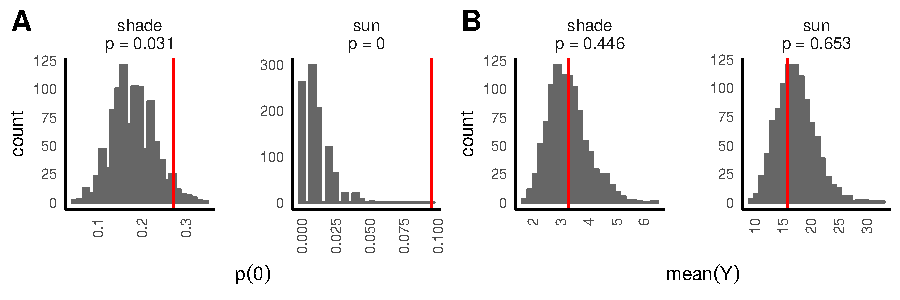
\includegraphics[scale = 0.8]{POIS_stip0_pp}
\caption{Predictive model checks of (\textbf{A}) proportion of zero counts $p(0)$ and (\textbf{B}) $\text{mean}(Y)$ for Poisson-only model of stipple counts. Observed values are indicated by red vertical lines.}
\label{fig:three}
\end{center}
\end{figure}

\subsubsection{ZI justification}

To justify our use of a ZINB model for the herbivory survey data, we first constructed Poisson-only models and compared them to global or habitat-specific ZI-Poisson models. (For the present illustration of our approach, we fit all models \emph{without} the leaf area term to improve convergence of the Poisson model with habitat-specific ZI terms; models \emph{with} this term are reported in the main text, and all direct comparisons can be found in the associated R code [\lib{https://github.com/phumph/habitat}]). Model checking (Figure \ref{fig:three}) reveals that the proportion of zeros under the fitted Poisson-only model simulations is not representative of the observed data ($p_{Z_0} = 0.03$ for shade sites, $p_{Z_0} \leq 10^{-3}$ for sun sites). In other words, the model simply fails to accurately represent the prevalence of damage across the dataset. When introducing a global zero-inflation term $\pi_0$, model fit greatly improves at the low end, as $p_{Z_0}$ increases to $0.85$ for sun sites (Figure \ref{fig:four}), and the overall goodness-of-fit improves substantially when judged by AICc ($\Delta\text{AICc} = -129$; Table S1). But we are still doing a poor job at capturing $p(0)$ in shade habitats, suggesting that habitat-specific estimates of $\pi^k_0$ may help. Indeed, modeling habitat-specific ZI improves the goodness-of-fit in shade habitats specifically ($p_{Z_0} \sim 0.40$ for both habitat types; Figure \ref{fig:five}). Including an additional model parameter is also statistically favored overall ($\Delta\text{AICc} = -1.8$; Table S1).

%%% PP CHECKS FOR POISSON MODEL, GLOBAL ZI
%%%%% Fig. S4
\begin{figure}[!htbp]
\begin{center}
%\setkeys{Gin}{width=0.33\textwidth}
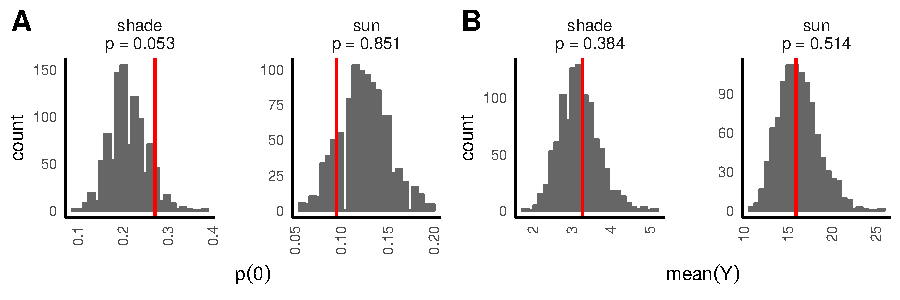
\includegraphics[scale = 0.8]{POIS_stip1_pp}
\caption{Predictive model checks of (\textbf{A}) proportion of zero counts $p(0)$ and (\textbf{B}) $\text{mean}(Y)$ for ZI-Poisson model of stipple counts with single global ZI parameter $\pi_0$. Observed values are indicated by red vertical lines.}
\label{fig:four}
\end{center}
\end{figure}

%%% PP CHECKS FOR POISSON MODEL, HABITAT-SPECIFIC ZI
%%%%% Fig. S5
\begin{figure}[!ht]
\begin{center}
%\setkeys{Gin}{width=0.33\textwidth}
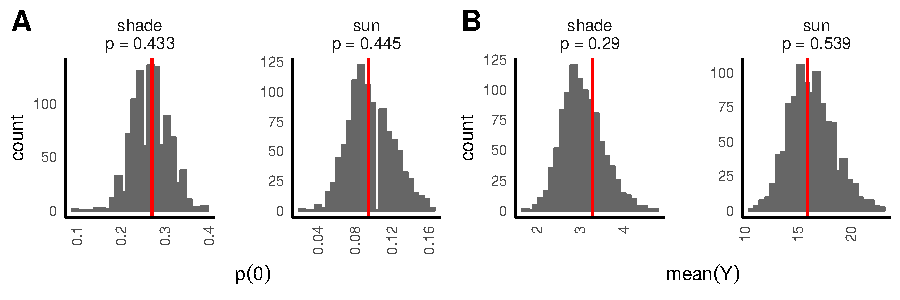
\includegraphics[scale = 0.8]{POIS_stip2_pp}
\caption{Predictive model checks of (\textbf{A}) proportion of zero counts $p(0)$ and (\textbf{B}) $\text{mean}(Y)$ for ZI-Poisson model of stipple counts with habitat-specific ZI parameters $\pi^{k}_0$. Observed values are indicated by red vertical lines.}
\label{fig:five}
\end{center}
\end{figure}

When we conduct a third predictive check to see how the improved model behaves at the high end, via calculating $\text{max}(Y)$, we see that the Poisson model fails to capture the difference between sites in the maximum counts observed (Figure \ref{fig:six}). 





\subsubsection{Zero-inflated negative binomial}

Model checking in this way shows that Poisson models, even when including habitat-specific ZI terms, can only take us so far in predicting the observed data across its entire range. The lack of fit of the \emph{same data used to estimate the model} indicates lack of flexibility in the model. Because we care about accurately modeling zero counts (i.e. damage prevalence) as well as damage abundance patterns, we explore a set of NB models in order to test whether introducing an additional latent parameter (NB dispersion parameter $\phi$) improves the ability of the model to capture habitat-specific patterns of herbivory.

%%% MAX(Y) FOR POISSON MODEL, HABITAT-SPECIFIC ZI
%%%%% Fig. S6
\begin{figure}[!t]
\begin{center}
%\setkeys{Gin}{width=0.33\textwidth}
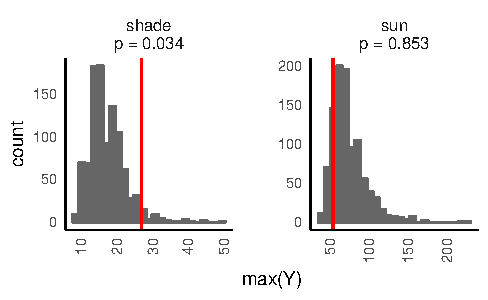
\includegraphics[scale = 0.8]{POIS_stip_2_max}
\caption{Predicted versus observed $\text{max}(Y)$ for ZI-Poisson model of stipple counts with habitat-specific ZI parameters $\pi^{k}_0$. Observed values are indicated by red vertical lines.}
\label{fig:six}
\end{center}
\end{figure}

Specifically, we compared NB-only to a series of NB models containing a single global ZI, habitat-specific ZI, as well as habitat-specific dispersion parameters with and without consideration of ZI (Table S1). Ultimately, the best model that gives both the lowest AICc (Table S1) as well as the most representative $p_Z$ estimates is a NB model with a global $\pi_0$ and habitat specific $\phi^k$. Specifically, this model performs at least as well as the two-level ZI-Poisson while also fitting better at the upper range, as indicated by the more representative range of $\text{max}(Y)$ (Figure \ref{fig:seven}).

This same analysis procedure was applied for the leaf miner data from the herbivory survey. These results are not displayed here but can be found in the \textbf{R} scripts in the \lib{github} repository associated with this manuscript (\lib{https://github.com/phumph/habitat/}).

%%% BEST NB MODEL, HABITAT-SPECIFIC DISPERSION, GLOBAL ZI
%%%%% Fig. S7
\begin{figure}[!h]
\begin{center}
%\setkeys{Gin}{width=0.33\textwidth}
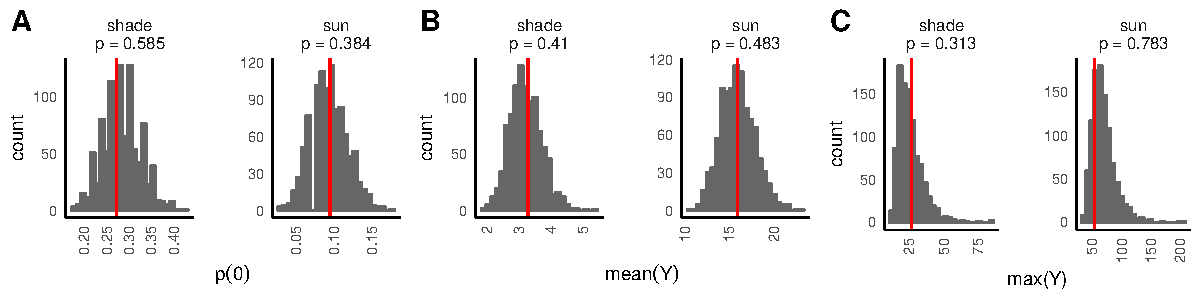
\includegraphics[scale = 0.7]{pp_stips_best_mod}
\caption{Predictive model checks for best-fitting ZINB model of stipple counts, with habitat-specific dispersion parameters $\phi^k$ and global ZI parameter $\pi_0$. Observed values are indicated by red vertical lines.}
\label{fig:seven}
\end{center}
\end{figure}

%capture zero-inflation in the data (particular in the sun sites) and how failing to take this into account distorts model fits at the upper end as well. Notably, the types of distortions that occur differ between shade and sun sites. Adding a zero-inflation term to a Poisson model will therefore not take care of both of these problems at once. We therefore move to zero-inflated negative binomial models. We first assess whether the inherent flexibility of the NB to accommodate extra-Poisson variance can solve the lower- and upper-range counts simultaneously, and then assess whether site type specific zero inflation or dispersion terms better-resolves the difference between how counts accrue at these two site types.

\newpage

%% TABLE S1
%% AICc values for all models considered in this section.
\begin{table}[!htbp]
\caption{Goodness-of-fit statistics for Poisson and NB models with and without accounting for ZI and dispersion.}
\centering
\small
\begin{tabular}{lllllllllll}
\toprule
family & $\Delta \text{AICc}$ & df & $\pi_0^{*}$ & NB $\phi^{*}$ & $p(0)^{shade}$ & $p(0)^{sun}$ & $\text{mean}(Y)^{shade}$ & $\text{mean}(Y)^{sun}$ & $\text{max}(Y)^{shade}$ & $\text{max}(Y)^{sun}$ \\
\midrule
NB & 0 & 7 & 1 & 2 & 0.59 & 0.38 & 0.41 & 0.48 & 0.31 & 0.78 \\
NB & 1.8 & 8 & 2 & 2 & 0.47 & 0.43 & 0.44 & 0.47 & 0.36 & 0.77 \\
NB & 19.3 & 7 & 2 & 1 & 0.44 & 0.45 & 0.34 & 0.56 & 0.09 & 0.93 \\
NB & 20.6 & 6 & 1 & 1 & 0.09 & 0.80 & 0.39 & 0.51 & 0.08 & 0.94 \\
NB & 63.3 & 5 & 0 & 1 & 0.07 & $<0.001$ & 0.46 & 0.62 & 0.32 & 0.99 \\
Poisson & 72.5 & 6 & 2 & $-$ & 0.43 & 0.45 & 0.29 & 0.54 & 0.03 & 0.85 \\
Poisson & 74.3 & 5 & 1 & $-$ & 0.05 & 0.85 & 0.38 & 0.51 & 0.05 & 0.90 \\
Poisson & 204.0 & 4 & 0 & $-$ & 0.03 & $<0.001$ & 0.45 & 0.65 & 0.20 & 0.94 \\
\bottomrule
\multicolumn{11}{l}{$^{*}$ 1 = single global parameter; 2 = habitat-specific parameters; 0 = not estimated; $-$ = not applicable}\\
\multicolumn{11}{l}{df = degrees of freedom}
\end{tabular}
\label{default}
\end{table}


\section{Herbivore choice tests I: Sun versus shade derived bittercress}

\subsection{Models for choice experiments}
Using NB generalized linear mixed models (GLMMs), we model variation in stipple and egg counts on plants arising from source habitat (sun versus shade) and leaf attributes (as fixed effects), as well as so-called structural random effects of plant ID nested within cage ID (i.e. replicate) to capture experimental design constraints that determine the level of independence among data points. We do not consider Poisson models in all subsequent analyses on the basis of far worse model fits observed for stipple and leaf mine data, above.

We also disfavored ZI models in principle because we assumed that \emph{S. nigrita} females had sufficient time to sample all available plants, and that variation in the intensity (rather than prevalence) of herbivory would drive most of our patterns. We did, however, consider whether including source habitat-specific estimates of $\phi_{k}$ empirically improved model fit, via model checking and AICc (see Results and Table 1 of main text).

Our mixed model for stipple and eggs counts, for both the whole-plant and detached leaf assays, takes the following form:

%%% Eq. 8
\begin{equation}
\text{log}(\mu_{ijk}) = \begin{cases}
	\alpha_0 + \beta x_i + \gamma_{(jk)} + \gamma_k & \text{if habitat = shade}.\\
    \alpha_0 + \alpha_1 + \beta x_i + \gamma_{(jk)} + \gamma_k & \text{if habitat = sun}.
  \end{cases}
\end{equation}

In this model, $\mu_{ijk}$ is the estimate for each leaf $i$, $\alpha_0$ and $\alpha_1$ are as in Eqn. 6, and $\beta$ is leaf position along stem (low to high) for the whole-plant model or leaf area (mm$^2$) for the detached leaf assay; finally, $\gamma_{k}$ represents a random effect of cage ID ($k$) and $\gamma_{(jk)}$ represents a random effect for plant ID $j$ nested within each level of cage ID $k$; $\gamma_{(jk)} \sim N(\gamma_{k},\tau^2_1)$ and $\gamma_{k} \sim N(0,\tau^2_2)$. Model comparisons and goodness-of-fit tests for analyses associated with this assay can be found in the \textbf{R} notebooks in our \lib{github} repository listed above.

\section{Herbivore choice tests II: Effects of light and temperature}

The NB model structures for this set of choice experiments were similar to those described above but with an expanded random effects structure. As for the previous herbivore choice models, all models described below are NB-only GLMMs. The choice trials in 2014 and 2015 were conducted slightly differently, which means that each year's data calls for slightly different random effects. We present the analyses of each dataset separately, then jointly.

\subsection{2014 Trials}

The 2014 field and lab trials were conducted in two temperature environments simultaneously, with one cage held in each. This gives a structure of temperature environment ($\gamma_{(lk)}$, $n=2$) nested within trial ($\gamma_{l}$, $n=6$ each for the 2014 field and lab assays). Nested within temperature environment is cage, but since we have only a single level of cage for each temperature environment per trial, this level is irrelevant for the 2014 dataset. However, we include side-of-cage ($\gamma_{(kj)}$, $n=2$; left or right, arbitrarily) to control for pseudo-replication at the level of the main treatment effect (i.e. Light environment, light versus dark), which was applied with randomization to the sides of each cage. Each random effect is $\sim N(0,\sigma_i^2)$. The full model is given below using the above notation for the random effects. The number of independent data points in the 2014 field and lab trials is 24 each (2 sides per cage, 1 cage per trial, 2 temperature settings per trial, and 6 trials).

%%% Eq. 9
\begin{equation}
\text{log}(\mu_{ijkl}) = \begin{cases}
\alpha_0 + \alpha_{1,i} + \alpha_{2,i} + \alpha_{12} + \beta x_i + \gamma_l + \gamma_{(lk)} + \gamma_{(kj)}
& \text{if Light = light, Temp = warm}\\
\alpha_0 + \alpha_{1,i} + \alpha_{2,i} + \beta x_i + + \gamma_l + \gamma_{(lk)} + \gamma_{(kj)} 	  		 
& \text{otherwise}.
\end{cases}
\end{equation}

We set the first levels of coefficients for the fixed effects of Light ($\alpha_{1,1} = \text{dark}$) and Temperature ($\alpha_{2,1} = \text{cool}$) equal to zero since these two states are incorporated into the Constant ($\alpha_0$, i.e. the reference level of the model). Our experiment was designed to allow us to fit an interaction term $\alpha_{12}$ which estimates how much the effect of Light is impacted by the Temperature environment (thus $\alpha_{12}$ has a single level). We fit models with the same structure for field and laboratory trials, and we consider condition-specific $\phi$ estimates when conducting model comparisons. Specifically, we estimated whether $\phi$ specific to light condition and/or temperature condition improved model fit by accounting for differential distributions of overdispersion analogous to Eq. 7 (with an additive [on the log scale] impact of temperature treatment).

\subsection{2015 Trials}
In the 2015 trials, we used bittercress leaves collected from both sun and shade habitats, and our randomization scheme ensured equal representation of sun- and shade-derived leaves across all treatments. We did this to test whether \emph{S. nigrita} would exhibit preference for shade-derived bittercress in the context of our temperature and light manipulations. In our analysis, we included leaf source (sun v. shade) as an additional fixed factor. Our model structure was thus

%%% Eq. 10
\begin{equation}
\text{log}(\mu_{ijkl}) = \begin{cases}
\alpha_0 + \alpha_{1,i} + \alpha_{2,i} + \alpha_{12} + \alpha_{3,i} + \beta x_i + \gamma_l + \gamma_{(lk)} + \gamma_{(kj)} 
& \text{if Light = light, Temp = warm}\\
\alpha_0 + \alpha_{1,i} + \alpha_{2,i} + \alpha_{3,i} + \beta x_i + \gamma_l + \gamma_{(lk)} + \gamma_{(kj)} 	  		 
& \text{otherwise}.
\end{cases}
\end{equation}

All coefficients are as in the 2014 trials above, except that the term $\alpha_{3,i}$ is for source habitat, and the first level ($\alpha_{3,1} = \text{shade}$) was set to $0$ and was thus incorporated into the intercept term $\alpha_0$. Thus, this model estimates only a single coefficient for the effect of habitat.

The experimental procedures also differed slightly in 2015. We placed two cages in one environmental chamber which was set to a single temperature per trial, and individual trials were conducted at different temperatures sequentially. This implies a structure of cage ($\gamma_{kl}$, $n=2$) nested within trial ($\gamma_{l}$, $n=5$), along with the side-of-cage nested within cage ($\gamma_{(kj)}$, $n=2$). The number of independent data points in the 2015 trials is thus 40 (2 sides per cage, 2 cages per room, 10 trials [5 in each temperature regime]). While the model structure is the same as in Eqn. 8, the meaning of the random effects (and their coding in the design matrix) are slightly different. Below we discuss how we reconciled the random effects to analyze both years' data together.

\subsection{Combined 2014-2015 Analysis}

We reconcile the slight distinctions between 2014 and 2015 datasets by including trial-year as a composite random effect, now re-coded to reflect each experiment conducted in a given room (compared to a trial containing two separate temperature settings, as in the 2014-only analysis). Nested within the new trial factor is cage, which has n = 1 for 2014 and n = 2 for 2015; side-of-cage is modeled in the same way as above. This model structure is now identical to Eqn. 10.

For the combined analysis, we drop the term for plant source habitat ($\alpha_3$) since the 2014 trials were not designed to examine plant source habtat. Additionally, we model both a continuous and discrete versions of the Temperature factor: the discrete model is the same as Eqn. 8, while in the continuous form, $\alpha_{2,j}$ is replaced with $\beta_2 y_j$, where $y_j$ is the temperature measured at the level of cage for each trial separately (Appendix B, Fig. 2C). Additionally, the fixed interaction term $\alpha_{12}$ is now replaced with an interaction modeled by the expression $\beta_3 y_j (\alpha_{1,j})$, which captures how the effect of light ($\alpha_{1,j}$) changes as a function of cage temp ($y_i$); since $\alpha_{1,i}$ has one level (the first level is set to 0), estimating this interaction term $\beta_3$ adds only a single parameter to the model. The full model is thus:

%%% Eq. 11
\begin{equation}
\text{log}(\mu_{ijkl}) = \alpha_0 + \alpha_{1,i} + \alpha_{2,i} + \beta_1 x_i + (\beta_2 + \beta_3\alpha_{1,i})y_j + \gamma_l + \gamma_{(lk)} + \gamma_{(kj)}
\end{equation}

Because the full model with the continuous temperature interaction term ($\beta_3$) exhibited such a poor fit to the data as judged by AIC (see below), we report the coefficient estimates for the nested model containing only the additive effect of the continuous temparture term ($\beta_2$; Table S2).


%%%%%%%%%%%%%%%%%%
%%%% TABLE S4 %%%%
%%%%%%%%%%%%%%%%%%
\begin{table}[!htp]
\begin{center}
\begin{small}
\caption{Coefficient estimates for all light--temp choice experiments.} 
\centering
\begin{tabular}{l@{} D{.}{.}{4.6}@{} D{.}{.}{4.5}@{} D{.}{.}{5.6}@{} D{.}{.}{5.6}@{} D{.}{.}{5.4}@{} D{.}{.}{4.6}@{} }
\toprule
& \multicolumn{5}{c}{Stipples}  & \multicolumn{1}{c}{Eggs} \\
\cline{2-6}\cline{7-7}\\
& \multicolumn{1}{c}{Field (2014)} & \multicolumn{1}{c}{Lab (2014)} & \multicolumn{1}{c}{Lab (2015)} & \multicolumn{1}{c}{Both years (1)} & \multicolumn{1}{c}{Both years (2)} & \multicolumn{1}{c}{Lab (2015)} \\
\midrule
\textit{Fixed effects} & & & & & & \\
$\alpha_0$ (Constant)                          & -2.038^{***} & -2.514^{**} & 0.364       & -1.147      & -4.123    & -4.870^{***} \\
                                               & (0.603)      & (0.870)     & (0.885)     & (0.661)     & (2.162)   & (0.812)      \\
$\beta_1$ leaf width (\textit{mm})             & 0.068^{***}  & 0.063^{*}   & -0.003      & 0.033       & 0.031     & 0.054^{**}   \\
                                               & (0.012)      & (0.026)     & (0.022)     & (0.018)     & (0.017)   & (0.019)      \\
$\alpha_1,$ [light]                            &              & 1.792^{*}   & 2.160^{***} & 2.019^{***} & 2.321^{***}    & 3.598^{***}  \\
                                               &              & (0.838)     & (0.515)     & (0.470)     & (0.339)   & (0.537)      \\
$\alpha_2$ [warm]                              &              & 0.399       & -0.100      & 0.109       &           & 1.960^{**}   \\
                                               &              & (0.885)     & (0.880)     & (0.667)     &           & (0.650)      \\
$\alpha_{12}$ [light:warm]                     &              & 1.123       & 0.293       & 0.636       &           & -1.994^{**}  \\
                                               &              & (1.172)     & (0.718)     & (0.654)     &           & (0.628)      \\
$\alpha_{3}$ [sun]                             &              &             & -0.291      &             &           & -0.002       \\
                                               &              &             & (0.701)     &             &           & (0.19)       \\
$\beta_2$ [temp]                               &              &             &             &             & 0.149     &              \\
                                               &              &             &             &             & (0.102)  &              \\
% $\beta_3$ [light:temp]                         &              &             &             &             & NA     &              \\
%                                                &              &             &             &             & (0.096)   &              \\
\textit{Random effects} & & & & & & \\
$\tau^2_{kj}$ [trial/cage/side]              & 0.559        & 1.397       & 0.720       & 1.102       & 1.129     & 0.152        \\
$\tau^2_{lk}$ [trial/cage]                   & 0.000        & 0.099       & 2.451       & 1.687       & 1.587     & 0.170        \\
$\tau^2_{l}$ [trial]                         & 0.204        & 0.000       & 0.000       & 0.000       & 0.063     & 0.163        \\
$\tau^2_{m}$ [year]                          &              &             &             & 0.036       & 0.000     &              \\
\midrule
AIC                                            & 1152.4     & 874.4     & 2125.7    & 2995.8    & 2993.4  & 861.2      \\
%BIC                                           & 1183.738     & 905.757     & 2161.594    & 3040.426    & 3084.345  & 897.044      \\
Log Likelihood                                 & -567.2     & -428.2    & -1053.9   & -1487.9   & -1487.7 & -421.6     \\
Num. obs.                                      & 240          & 240         & 398         & 638         & 638       & 398          \\
\bottomrule
\multicolumn{7}{l}{\scriptsize{$^{***}p<0.001$, $^{**}p<0.01$, $^*p<0.05$}}
%\multicolumn{7}{l}{Note that coefficient estimates for these models do not include estimation of condition-specific $\phi$.}
\end{tabular}
\label{table:coefficients2}
\end{small}
\end{center}
\end{table}

%
%\subsection{Model Selection}
%
%In the main text, we report the results from the NB GLMMs fit to the 2014 and 2015 datasets (separately) using \textbf{R} package \lib{glmmTMB}. The full results for the combined analysis is displayed in Table S3.

%
%For the 2014 and 2015 datasets, we also analyzed a series of nested models to evaluate the relative performance of simpler nested models (Table S5-S7). We calculated AIC and also performed likelihood ratio tests (not shown, but can be calculated from reported log likelihoods), which agreed with $\Delta\text{AIC}$ results. Additionally, we evaluated overall model fit for the fixed effects-only portion with $R^{2(M)}_{GLMM}$ and for all model terms combined with $R^{2(C)}_{GLMM}$ using which were calculated as derived in \cite{Nakagawa13a} using \textbf{R} package \lib{piecewiseSEM} \cite{Lefcheck16a}. The models reported in the main text are not typically the best model as judged by AIC. Nonetheless, we report the more complex models in the main text so that the coefficient estimates for all terms are available to the reader; the terms retained in the models with lowest AIC in Tables S5-S7 correspond to those with statistically significant ($p<0.05$) coefficient estimates in the main text tables.
%
%%%%%%%%%%%%%%%%%%%
%%%%% TABLE S5 %%%%
%%%%%%%%%%%%%%%%%%%
%%\newpage
%\begin{tiny}
%\begin{table}[!htbp]
%\caption{Model comparisons for different fixed effect combinations: 2014.} 
%\centering
%%\resizebox*{!}{\dimexpr\textheight-2\baselineskip\relax}{%
%\begin{tabular}{llccccc}
%\toprule
%Dataset & Fixed effects & $R^{2(M)}_{GLMM}$ & $R^{2(C)}_{GLMM}$ & AIC & $\Delta AIC$ & log Lik \\ 
%\midrule
%\textit{2014 Field} & $\alpha_0$ & 0.00 & 0.85 & 1190.05 & 37.98 & -590.03 \\ 
% (stipples) & $\alpha_0, \beta$ & 0.31 & 0.91 & 1158.50 & 6.43 & -573.25 \\ 
% & $\alpha_0, \beta, \alpha_1$ & 0.52 & 0.91 & 1152.07 & \textbf{0.00} & -569.03 \\ 
% & $\alpha_0, \beta, \alpha_1, \alpha_2$ & 0.54 & 0.91 & 1152.81 & 0.75 & -568.41 \\ 
% \multicolumn{1}{r}{$\longrightarrow$} &  $\alpha_0, \beta, \alpha_1, \alpha_2, \alpha_{12}$ & 0.58 & 0.90 & 1152.41 & 0.34 & -567.21 \\ 
%
%\textit{2014 Lab} & $\alpha_0$ & 0.00 & 0.86 & 888.57 & 15.23 & -439.29 \\ 
%(stipples) & $\alpha_0, \beta$ & 0.06 & 0.87 & 883.03 & 9.69 & -435.52 \\ 
% &  $\alpha_0, \beta, \alpha_1$ & 0.41 & 0.86 & 873.84 & 0.50 & -429.92 \\ 
% & $\alpha_0, \beta, \alpha_2$ & 0.12 & 0.87 & 883.41 & 10.08 & -434.71 \\ 
% &  $\alpha_0, \beta, \alpha_1, \alpha_2$ & 0.47 & 0.85 & 873.34 & \textbf{0.00} & -428.67 \\ 
%\multicolumn{1}{r}{$\longrightarrow$} &  $\alpha_0, \beta, \alpha_1, \alpha_2, \alpha_{12}$ & 0.48 & 0.85 & 874.43 & 1.09 & -428.22 \\ 
%%  &  12 & 0.44 & 0.86 & 874.61 & 1.28 & -429.31 \\ 
%%  &  13 & 0.49 & 0.85 & 873.85 & 0.51 & -427.93 \\
%\bottomrule
%\small\textit{Notes:} & \multicolumn{6}{r}{\small$\Delta AIC$ is each model minus model with lowest AIC.} \\
%					 & \multicolumn{6}{r}{\small$\longrightarrow$ indicates model reported in main text, Table 3.} \\
%\end{tabular}
%\end{table}
%\end{tiny}
%
%%%%%%%%%%%%%%%%%%%
%%%%% TABLE S6 %%%%
%%%%%%%%%%%%%%%%%%%
%%\newpage
%\begin{tiny}
%\begin{table}[!htbp]
%\caption{Model comparisons for different fixed effect combinations: 2015.} 
%\centering
%%\resizebox*{!}{\dimexpr\textheight-2\baselineskip\relax}{%
%\begin{tabular}{llccccc}
%\toprule
%Dataset & Fixed effects & $R^{2(M)}_{GLMM}$ & $R^{2(C)}_{GLMM}$ & AIC & $\Delta AIC$ & log Lik \\ 
%\midrule 
%\textit{2015 Lab} & $\alpha_0$ & 0.00 & 0.95 & 2140.95 & 19.06 & -1065.48 \\ 
%(stipples) & $\alpha_0, \beta$ & 0.00 & 0.95 & 2142.79 & 20.90 & -1065.40 \\ 
% & $\alpha_0, \beta, \alpha_1$ & 0.28 & 0.95 & 2121.89 & \textbf{0.00} & -1053.94 \\ 
% &  $\alpha_0, \beta, \alpha_2$ & 0.00 & 0.95 & 2144.78 & 22.89 & -1065.39 \\ 
% &  $\alpha_0, \beta, \alpha_1, \alpha_2$ & 0.28 & 0.95 & 2123.88 & 1.99 & -1053.94 \\ 
% & $\alpha_0, \beta, \alpha_1, \alpha_2, \alpha_{12}$ & 0.29 & 0.95 & 2124.47 & 2.59 & -1053.24 \\ 
% &  $\alpha_0, \beta, \alpha_1, \alpha_2, \alpha_3$ & 0.29 & 0.95 & 2126.26 & 4.37 & -1053.13 \\ 
%\multicolumn{1}{r}{$\longrightarrow$} & $\alpha_0, \beta, \alpha_1, \alpha_2, \alpha_{12}, \alpha_3$ & 0.28 & 0.95 & 2125.72 & 3.83 & -1053.86 \\ 
%%  &  22 & 0.29 & 0.95 & 2124.48 & 2.59 & -1053.24 \\ 
%%  &  23 & 0.29 & 0.95 & 2126.40 & 4.51 & -1053.20 \\ 
%% \textit{2015 Lab} &  24 & 0.00 & 0.64 & 908.39 & 47.22 & -449.19 \\ 
%(eggs) & $\alpha_0$ & 0.00 & 0.64 & 908.39 & 47.22 & -449.19 \\ 
% & $\alpha_0, \beta$ & 0.02 & 0.64 & 902.03 & 40.86 & -445.01 \\ 
% & $\alpha_0, \beta, \alpha_1$ & 0.43 & 0.64 & 867.95 & 6.78 & -426.97 \\ 
% & $\alpha_0, \beta, \alpha_2$ & 0.05 & 0.65 & 902.43 & 41.26 & -444.21 \\ 
% & $\alpha_0, \beta, \alpha_1, \alpha_2$ & 0.46 & 0.65 & 867.88 & 6.71 & -425.94 \\ 
% & $\alpha_0, \beta, \alpha_1, \alpha_2, \alpha_{12}$ & 0.56 & 0.68 & 861.17 & \textbf{0.00} & -421.58 \\ 
%& $\alpha_0, \beta, \alpha_1, \alpha_2, \alpha_3$ & 0.46 & 0.65 & 869.87 & 8.71 & -425.94 \\
%\multicolumn{1}{r}{$\longrightarrow$} & $\alpha_0, \beta, \alpha_1, \alpha_2, \alpha_{12}, \alpha_3$ & 0.56 & 0.68 & 863.17 & 2.00 & -421.58 \\
%\bottomrule
%\small\textit{Notes:} & \multicolumn{6}{r}{\small$\Delta AIC$ is each model minus model with lowest AIC.} \\
%					 & \multicolumn{6}{r}{\small$\longrightarrow$ indicates model reported in main text, Table 3.} \\
%\end{tabular}
%\end{table}
%\end{tiny}
%
%%%%%%%%%%%%%%%%%%%
%%%%% TABLE S7 %%%%
%%%%%%%%%%%%%%%%%%%
%%\newpage
%\begin{tiny}
%\begin{table}[!htbp]
%\caption{Model comparisons for different fixed effect combinations: 2014--2015 combined} 
%\centering
%\begin{tabular}{llccccc}
%\toprule
%Dataset & Fixed effects & $R^{2(M)}_{GLMM}$ & $R^{2(C)}_{GLMM}$ & AIC & $\Delta AIC$ & log Lik \\ 
%\midrule
%\textit{Combined Lab} &  $\alpha_0$ & 0.00 & 0.93 & 3025.93 & 32.55 & -1506.97 \\ 
%(Stipples) &  $\alpha_0, \beta_1$ & 0.02 & 0.93 & 3022.43 & 29.04 & -1504.21 \\ 
%&  $\alpha_0, \beta_1, \alpha_1$ & 0.31 & 0.92 & 2993.43 & 0.04 & -1488.71 \\ 
%&  $\alpha_0, \beta_1, \alpha_2$ & 0.02 & 0.93 & 3023.84 & 30.45 & -1503.92 \\ 
%&  $\alpha_0, \beta_1, \alpha_1, \alpha_2$ & 0.32 & 0.93 & 2994.78 & 1.40 & -1488.39 \\
%&  $\alpha_0, \beta_1, \alpha_1, \alpha_2, \alpha_{12}$ & 0.32 & 0.93 & 2995.84 & 2.46 & -1487.92 \\ 
%&  $\alpha_0, \beta_1, \alpha_1, \beta_2$ & 0.35 & 0.92 & 2993.38 & \textbf{0.00} & -1487.69 \\ 
%&  $\alpha_0, \beta_1, \alpha_1, \beta_2, \beta_3$ & 0.35 & 0.92 & 2994.27 & 0.89 & -1487.14 \\ 
%\bottomrule
%\small\textit{Notes:} & \multicolumn{6}{r}{\small$\Delta AIC$ is each model minus model with lowest AIC.} \\
%\end{tabular}
%\end{table}
%\end{tiny}

%%% REFERENCES
\newpage
\bibliographystyle{plain}
\bibliography{stat_sup.bib}{}

\end{document}
